% Author: Izaak Neutelings (July 2018)
\documentclass[border=3pt,tikz]{standalone}
\usepackage{amsmath}
\usepackage{tikz}
\tikzset{>=latex} % for LaTeX arrow head
%\usepackage{xcolor}
%\colorlet{charge+}{blue!80!white}
\tikzstyle{charge0}=[top color=green!80!black!50,bottom color=green!80!black,shading angle=20]
\tikzstyle{charge+}=[top color=red!50,bottom color=red!70!black,shading angle=20]
\tikzstyle{charge-}=[top color=blue!50,bottom color=blue!80,shading angle=20]
%\tikzstyle{charge+}=[thin,ball color=blue!60,shading angle=-10]
%\tikzstyle{charge-}=[thin,ball color=red!85,shading angle=-10]
%\tikzstyle{charge0}=[thin,ball color=green!80!black!80,shading angle=-10]



\def\d{0.8}
\def\R{1.0}
\def\N{{1.04*(\R+\d)}}


\begin{document}
\Large


% CUPPER ATOM
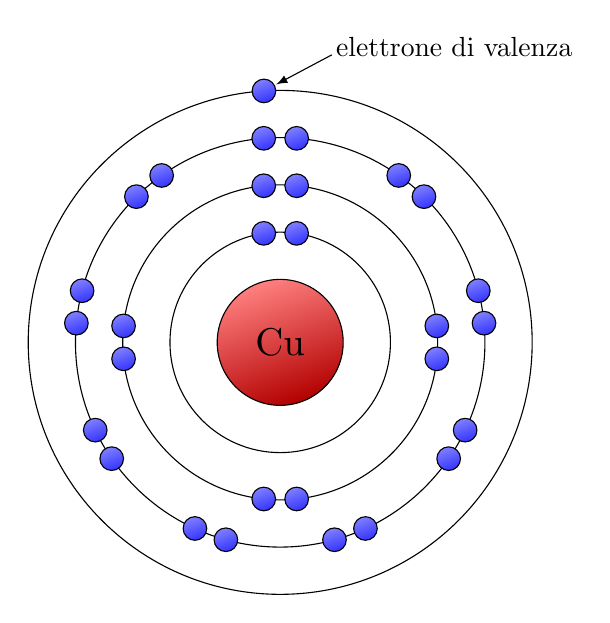
\begin{tikzpicture}
    \def\R{0.8}
    \def\a{0.6}
    \def\re{0.15}
    \def\dang{12}

    % NUCLEUS
    \draw[charge+] (0,0) circle (\R) node[scale=1.4] {Cu};

    % ORBITAL
    \foreach \i/\No [evaluate={\r=\R+\i*\a;}] in {1/1,2/4,3/9}{
            \draw (0,0) circle (\r);
            \foreach \j [evaluate={\ang=90+\j*360/\No;}] in {1,...,\No}{
                    \draw[charge-] ( \dang/\r+\ang:\r) circle (\re);
                    \draw[charge-] (-\dang/\r+\ang:\r) circle (\re);
                }
        }

    % VALENCE ELECTRON
    \draw (0,0) circle (\R+4*\a);
    \draw[charge-] (93.7:\R+4*\a) circle (\re) coordinate (V);
    \draw[<-] (V) ++ (28:1.18*\re) --++ (28:0.8) node[below=2,above right=-2] {elettrone di valenza};

\end{tikzpicture}


% COMPOSITE MODEL
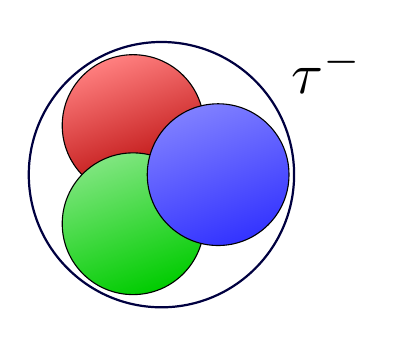
\begin{tikzpicture}[scale=0.9]

    \coordinate (O)  at (  0, 0);
    \coordinate (D1) at (  0:\d);
    \coordinate (U1) at (120:\d);
    \coordinate (U2) at (240:\d);
    \coordinate (L)  at ( 30:\N);

    \draw[charge+] (U1) circle (\R);
    \draw[charge0] (U2) circle (\R);
    \draw[charge-] (D1) circle (\R);
    \draw[thick,blue!25!black] (O) circle (\N);
    \node[above right=-2,scale=2.1] at (L) {$\tau^-$};

\end{tikzpicture}


\end{document}